\documentclass {article}

\usepackage [utf8]{inputenc}

\usepackage {graphicx}

\renewcommand {\contentsname} {Menù}

\title {{\Huge Bitcoin, blockchain, crypto}}

\author {Carlomaria Occhipinti\\Liceo Scientifico Arturo Tosi}

\date {Giugno 2018}



\begin {document}

\maketitle

\newpage

\tableofcontents

\pagenumbering {gobble}

\newpage

\pagenumbering {arabic}



\section {Le origini del Bitcoin e il suo obiettivo PE RPRIMA OCASà}



nasce.... eprche........

Satoshi creò una valuta con numerosi pregi: ELENCO PUNTATO decentralizzata, anonima, veloce, ......?, universale

Spiegare elenco puntato.



\section {Blockchain: cos'è e come funziona}



La tecnologia rivoluzionaria utilizzata dal Bitcoin e da tutte le altre criptovalute è chiamata Blockchain (technology?).

Come suggerisce il nome, "blockchain" indica/significa una catena di blocchi.

Come la figura mette bene, tutte le transazioni di BTC sono permanentemente, incancellabilmente memorizzate nella Blockchain.

Volendo, posso vedere quanti bitcoin X ha spedito a Y. Ogni blocco, infatti, contiene informazioni su tutte le transazioni che sono state compiute nell'intervallo di tempo in cui quel blocco rimane "attivo".

In che senso "rimane attivo"? Quando un blocco diventa "inattivo"?

Mi tocca introdurre il concetto di "mining".



\subsection {Mining}



I blocchi, per poter essere "risolti" vengono "minati" dai cosiddetti "miners", dei computer specializzati a risolvere un certo tipo di algoritmo.

Algoritmo, perchè il processo di mining consiste esclusivamente nella matematica.

Il mining consiste in (l'ho gia detto 3 o 4 volte lol) indovinare la "parola chiave", chiamata "hash" (non la droga xd) che serve per risolvere un blocco.

Questa parola chiave è una stringa lunga circa XXXX caratteri.

Come uno può immaginare, indovinarla è molto difficile, infatti i miners lavorano a velocità esorbitanti.

Il miner di Bitcoin che si usa oggi lavora a 13.5 TH/s (tera-hash al secondo), ovvero PIU DI TREDICI TRILIONI DI TENTATIVI IN UN SECONDO.

Questi apparecchi sono molto costosi (minimo 1000 per unità) e utilizzano un'elevata quantità di energia elettrica per funzionare.

Perchè, allora, c'è gente che spende tutti questi soldi per fare il lavoro di mining? PROOFG  OF WORK SOMEWHERE AAAAAAAAAAAAAAAAAAAAAAAA

Ebbene, quando si "risolve" un blocco, il miner riceve una quantità pari a 12.5 Bitcoin, oggi pari a circa 90000 euro (parlare di halving whand?). Quasi mai, però, i 12 btc finiscono a una singola persona: indovinare la stringa che mina il block è estremamente difficile! Per questo esistono le "pool" di mining, dei siti in cui più miners uniscono gli sforzi per risolvere il blocco. Una volta indovinato, la ricompensa si spartisce fra tutti i miner, in base a quanto ciascuno si è impegnato per trovarla.

Torniamo a noi, cosa succede quando il blocco è minato, e si passa a quello successivo? Tutte le transazioni che si sono accumulate nel blocco precendente (quello che i miner stavano cercando di risolvere) vengono confermate, e impiantate nella blockchain. Per questo, una transazione è considerata conclusa quando si passano almeno 3 blocchi dopo quello in cui è stata iniziata.

3 perchè.............??

è così che funziona la blockhain bla b la



\subsubsection {Gli effetti del mining sull'ambiente}



eh è brutto lol, ma non quanto i banker skifosi xd



\subsection {How and where Bitcoin is stored}



\subsubsection {Wallets}



A wallet is the software used to make the user interact with their coins / that makes you send and recieve Bitcoin. It can be an app for smartphones, a program on a computer, or even an online service.

While wallets are the software itself, they are not the "place" where bitcoins are stored. The coins are stored in addresses, a string of x characters that starts with either 1, 3, or bc1 (I'll explain the differences between those later). An address can be seen as an IBAN address, or even an email address.

Bitcoin can be stored in two different ways: cold wallets and hot wallets.



\paragraph {Cold wallets}



Cold wallets are..



\paragraph {Hot wallets}



Hot wallets are...



\paragraph {Hardware wallets}



Really neat cus...



\subsubsection {Keys}



Every Bitcoin address is associated with a private key.

A private key, as the name suggests, is a key that gives full access to the coins stored in its address.



\subsubsection {Seeds}



New (as in...............)Hot wallets work with SEEDS: a seed is kind of a password that gives you access to your coins (stored online?) a seed is typically 12 or 15 english words that, when put into the wallet ocnfiguration makes magically appear all your coins. That's the reason why "seed stealing" is the most common tactic of stealing funds: with a bunch of apparently useless words, new users can be tricked into sending them to a scammer who quickly steals alltheir coins and runs away.

A seed is associated with x different Bitcoin addresses, for privacy purposes: despite not being linked with private information such as name, surname and address, we saw that every transaction is permanently written into the blockchain, and anyone can see any address' current BTC balance. For this reason, having different addresses helps in making the user less traceable (SCRIVERE PRIMA COME SI POSSONO TRACCIARE), as it's impossible to link the seed's different addresses. Wallets that use seeds still report the total balance as the sum of funds in each seed's address.



PARLARE DI ALTRI ALGORITMI E ALTRE VALUTE, AJCHE SE PARLO DOPO DELLE ALTE VALUTE, ONON SO CSAO FARE AOITUO.....



\subsection {Cuscinetti / integrazioni}



Il bitcoin è la prima criptovaluta mai creata, e questo la rende anche la più vecchia e obsoleta sotto il punto di vista tecnologico. Come vedremo in seguito, infatti, oggi esistono molte valute che riducono, o in certi casi sistemano i principali "problemi" del Bitcoin.



\subsubsection {Segregated Witness}



Segregated Witness (comunemente abbreviato in SegWit) è una roba che riduce le tasse



\subsubsection {Lightning Network}



ANche LN lol



\section {Utilizzare Bitcoin}



Ho notato che nonostante se ne parli sempre di più in televisione e su internet, il Bitcoin è sempre visto come un concetto astratto, un'entità misteriosa di cui non si sa esattamente come si usa, dove si prende, e in cosa si spende.



\subsection {Come ottenere criptovaluta}



\subsubsection {Exchange}



Il metodo più veloce e utilizzato è quello di acquistarlo su un sito di exchange (come si dice in ita??). Esistono moltissimi siti che permettono di acquistare Bitcoin con bonifico bancario o semplicemente con una carta di credito, come se si stesse acquistando un oggetto.

Coinbase è by far l'exchange più famosa del mondo. Basta aprire un account, collegare il proprio conto o la carta di credito, e compare btc è questione di secondi.

Una volta acquistato, è consigliabile spostare i propri bitcoin su un "wallet" indipendente dal sito dell'exchange. Coinbase è la più sicura e attendibile, ma ci sono stati tragici episodi di exchange hacked, mln lost. (v sub...)



\subsubsection {ATMs}



Esistono dei veri e propri bancomat in cui anzichè prelevare soldi dal proprio conto bancario è possibile acquistare e vendere criptovalute. Sono comodi, veloci ed anonimi, ma c'è sempre il rischio di venire derubati tramite forza fisica; si paga un bonus per la comodità (fee, higher trade price) e al giorno d'oggi sono ancora molto poco diffuse. Si può trovare una mappa online con la posizione di questi ATM in tutto il mondo su https://nuiasbdiasnd.lol.



\subsubsection {Mining}



Come spiegato in precedenza, il processo di mining porta i miners a guadagnare criptovalute, che possono essere venudre (se parlassi pirma delle altre valute??) per btc, o soldi veri e propri.

Nonostante i costi dell'equipaggiamento di minning e dell'elettrricità utilizzata, i miner ricavano comunque un profitto dai coin che guadagnano. Ovvio che per "the average Joe" il mining è "out of their league", ma è certamente un modo valido per ottenere dei coin



\subsubsection {Vendere roba}



Se si vendfe qualcosa su i nternet o in real live si può comunicare ai clienti che è preferibile accettare pagamenti in bvitoicnoin.



\subsection {Spendere Bitcoin}



Il Bitcoin è una valuta relativamente nuova, nata neanche 10 anni fa, e il fatto che utilizza una tecnologia sconosicta prima d'ora, limita il ---- è temuta

Nonostante ciò, sempre più negozi online e "in vita reale" stanno cominciando ad accettare criptovalute come forma di pagamento. Esiste una pagina (FARE LINK DIDASCALIA IN BASSSO https://99bitcoins.com/who-accepts-bitcoins-payment-companies-stores-take-bitcoins/) con una lista che comprende (ma non è limitata a) luoghi e siti web sui quali si può pagare in bitcoin.

La lista comprende un numero limitato di --- come chiamarli?, ma in realtà sono molti di più.

Tra i più rilevanti ci sono: ELENCO PUNTATO





\section {Non solo Bitcoin}



Esistono numerosissime criptovalute. Il sito https://coinmarketcap.com ne lista X00. Ritengo indispensabile spendere almeno qualche pagina a discutere/?????? delle valute più rilevanti, perchè a common misconception is that Bitcoin is the only cryptocurrency. This is simply not true. Tutte le criptovalure che non sono Bitcoin prendono il nome di Altcoin, "alternative coin".



\subsection {Ethereum}



get vitalik on ze line xd



\subsection {Litecoin}



arise chickun lal



\subsection {Monero}



Monero è un altcoin creato nel



\subsection {Nano}



BEST COIN



\subsection {Stellar?}



idk much tbh smh



\subsection {Bitcoin "hard forks"}



La blockchain del Bitcoin "originale" può essere clonata indefinitamente. Chiunque può prendere il codice sorgente del Bitcoin, applicarci qualche modifica e mandarlo "live", rendendo disponibili dei wallet al download e impiegando qualche miner per processare le transazioni del "nuovo" bitcoin.



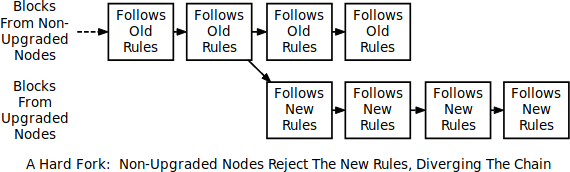
\includegraphics [width = 10cm] {media/hard_fork.png}



Oggi esistono numerosissime "fork" del Bitcoin: Bitcoin Gold, Bitcoin Candy, Bitcoin Private, Bitcoin Unlimited, Bitcoin Super... Persino Bitcoin Pizza e Bitcoin God.

Quasi tutti i fork vengono visti come delle truffe, come valute che non possiedono nulla di nuovo rispetto all'originale Bitcoin, ma viene sempre data attenzione perché chiunque possiede Bitcoin il momento in cui la blockchain è stata clonata, entra automaticamente in possesso del coin della fork. Se un indirizzo ha il bilancio di X BTC PRIMA che venga lanciato il clone di BTC, per esempio Bitcoin Top (BTT) a quell'indirizzo sarà anche associato X BTT.

Per poter ottenere effettivamente tutti i coin che l'indirizzo "possiede", è necessario scaricare il software di wallet del coin di fork e inserire la private key dell'indirizzo con su il coin di fork.

Verrà generato un nuovo indirizzo completamente diverso, però con il bilancio di X FKC.

Abbiamo visto prima che la private key dà accesso a tutti i fondi presenti sull'indirizzo a chiunque ne entri in possesso, eppure per ottenere i Fork siamo costretti ad inserirla in un software sconosciuto (perchè quasi tutti i fork non hanno alcuna reputazione: saltano fuori con siti web senza preavviso).

Per evitare che un qualche malintenzionato sfrutti la sbadataggine dell'utente e rubi tutti i suoi bitcoin, è bene che I fondi vengano mossi a un altro indirizzo.

Infatti, sarà comunque possibile prelevare i fkc dal vecchio indirizzo ora svuotato, e non si ha nulla da perdere se qualcuno riesce a rubarci la private key: l'indirizzo ha su 0 BTC.



\subsubsection {Roger Ver e la truffa di "Bitcoin Cash"}



Bitcoin Cash è by far l'hard fork più popolare di tutte, al quarto posto (!) in capitalizzazione di mercato. Come mai è l'unica che ha raggiunto un prezzo così elevato?

Roger K. Ver è un imprenditore americano che fin dai primi anni della nascita del Bitcoin è stato coinvolto nella scena delle criptovalute, finanziando progetti (?) e tenendo discorsi (??).

Da Agosto 2017, però, quando è stato lanciato Bitcoin Cash, Roger è stato l'esponente principale per il / del marketing di questa valuta. BCH è nato in Cina, infatti i suoi "CEO" sono cinesi, e Roger dev'essere stato impiegato per fare propaganda a BCH.

Tutto ciò non sembra alcunché di preoccupante: è normale se un imprenditore pubblicizza i propri investimenti sperando di ricavare più guadagni, (nel caso che...) ed è normale che sviluppatori paghnio uno abile a parlare e a pubblcizzare un prodotto. è così che funziona il marketing.

Quella di Roger, però, è una spietata propaganda anti-Bitcoin (BTC) e pro-BCH (Bitcoin Cash), che spesso e volentieri arriva alla censura, alle bugie più false e alla corruzione di persone.

La tesi base che accomuna Roger e tutti i fan di BCH (pagati o no non si sa), è quella che BCH introduce delle modifiche al codice di Bitcoin che rendono le transizioni notevolmente più veloci, sicure e con una tassa di transazione inferiore. Bitcoin Cash infatti ha come principale differenza un'incrementata dimensione del blocco (V. 1.2), che anzichè limitarsi a 1MB arriva fino a 12MB (come abbiamo visto, ogni transazione pesa tot kb. essendo il blocco più grande può farci stare più transazioni, senza "intasarsi").

Il team di sviluppatori di Bitcoin si ostina a mantenere la dimensione del blocco a 1MB, perchè i blocchi di maggiore dimensioni sono *ancora* più difficili da minare. Una difficoltà così elevata di mining porta necessariamente a una centralizzazione dell'hashing power, che va contro il concetto di Bitcoin e di criptovalute in generale (valute decentralizzate, internazionali, v 1.1).

Roger è entrato in possesso del sito bitcoin.com, che su numerose pagine (tra cui quella in fig. 5) ripete come BCH è una versione aggiornata di BTC. Una cosa che irrita la stragrande maggioranza delle persone è il fatto che su bitcoin.com il Bitcoin originale, BTC, è chiamato Bitcoin Core. Il nome Bitcoin Core, paragonato a Bitcoin Cash, fa sembrare le due valute due alternative sullo stesso livello, invece uno (BCH) è un clone dell'originale (BTC). (LAWSUIT BCH = BITCOIN)

bitcoin.com, essendo il secondo risultato su google perl la ricerca "bitcoin", ha portato molte persone nuove nel mondo delle fcriptovalòute che cercavano di acquistare dei Bitcoin ad acquistare BCH anziché BTC.

Ver possiede anche l'account twitter @bitcoin, che svolge le stesse opere di propaganda di bitcoin.com



\section {Bitcoin oggi}



si sta usando un po', blabla



\subsection {Lo stato attuale dell'adozione}



Sempore più negozi, serivzi, droga.....



\subsubsection {Il villaggio in Austria.. come si chiama?}



è bellus



\subsection {Il boom del 2017: cause e conseguenze}



MOOON BOIS LAMBO LETS GO



\subsubsection {La ricorrenza dei "crash" dei mercati}



*foto che compara*, succede tante voplte, hodl godl podl.



\subsection {Controversie}



Il Bitcoin e le criptovalute in generale sono frequentemente soggetto di controversie. La nuova tecnologia della blockchain è criticata da molti imprenditori, e numerosissime truffe girano intorno all'anonimità della valuta (wut lol)



\subsubsection {Mt. Gox}



Mt. Gox è il primo grande sito di exchange di Bitcoin, creato a Tokyo, JP nel 2013.

Ai tempi il Bitcoin aveva un valore ben più basso del €9000 di oggi: il giorno in cui l'hack è avvenuto un bitcoin valeva "solo" eur500.



\subsubsection {Bitconnect}



Bitconnect è un altcoin che aumentava del x% i profitti di chiunque ne possedesse un po'.

Non era ben chiaro chi fosse il creatore, e molti erano già dubiosi del claim di arricchire magicamente chiunque ne comprasse.

Nel .. 2017 il prezzo di Bitconnect è crollato da X a Y. Si è scoperto che l'intero progetto Bitconnect non era altro che un' "exit scam", una truffa in cui i truffatori spariscono improvvisamente, lasciando gli investitori a mani vuote. In particolare Bitconenct è stato uno schema Ponzi, un tipo di truffa in cui il truffatore promette guadagni a chiunque si indebitasse con lui, per poi sparire. Il nome Ponzi deriva da Charles Ponzi, un italo-americano che si arricchì notevolmetne negli anni '30(??????) compiendo ripetutamente questo tipo di truffa.

Oggi tutti coloro coinvolti nel pubblicizzare Bitconnect, soprattutto Youtuber (spiegare chi sono?) sono sotto investigazione



\section {Il futuro delle criprtovalute}



Come si può vedere dalla figura, nel 2018 ci troviamo alla primissima fase dell'adozione di questa nuova tecnologia.







\end {document}
